\chapter{Project evaluation}

\epigraph{And}{Once in a Lifetime \\ Talking Heads, 1981}

\section{Overview}

This thesis lives as a PDF document at the MIT library, as a software library with examples for Arduino, and as repositories on GitHub with all the source code and history of the project.

\section{Digital release}

The repositories are hosted on GitHub, to promote collaboration, and people can file issues and pull requests.

GitHub repository

Arduino library

PDF zine for explaining, reference as the PDF booklet for monome norns

\section{Audience engagement}


\section{Workshop}

\begin{figure}[h]
	\centering
	  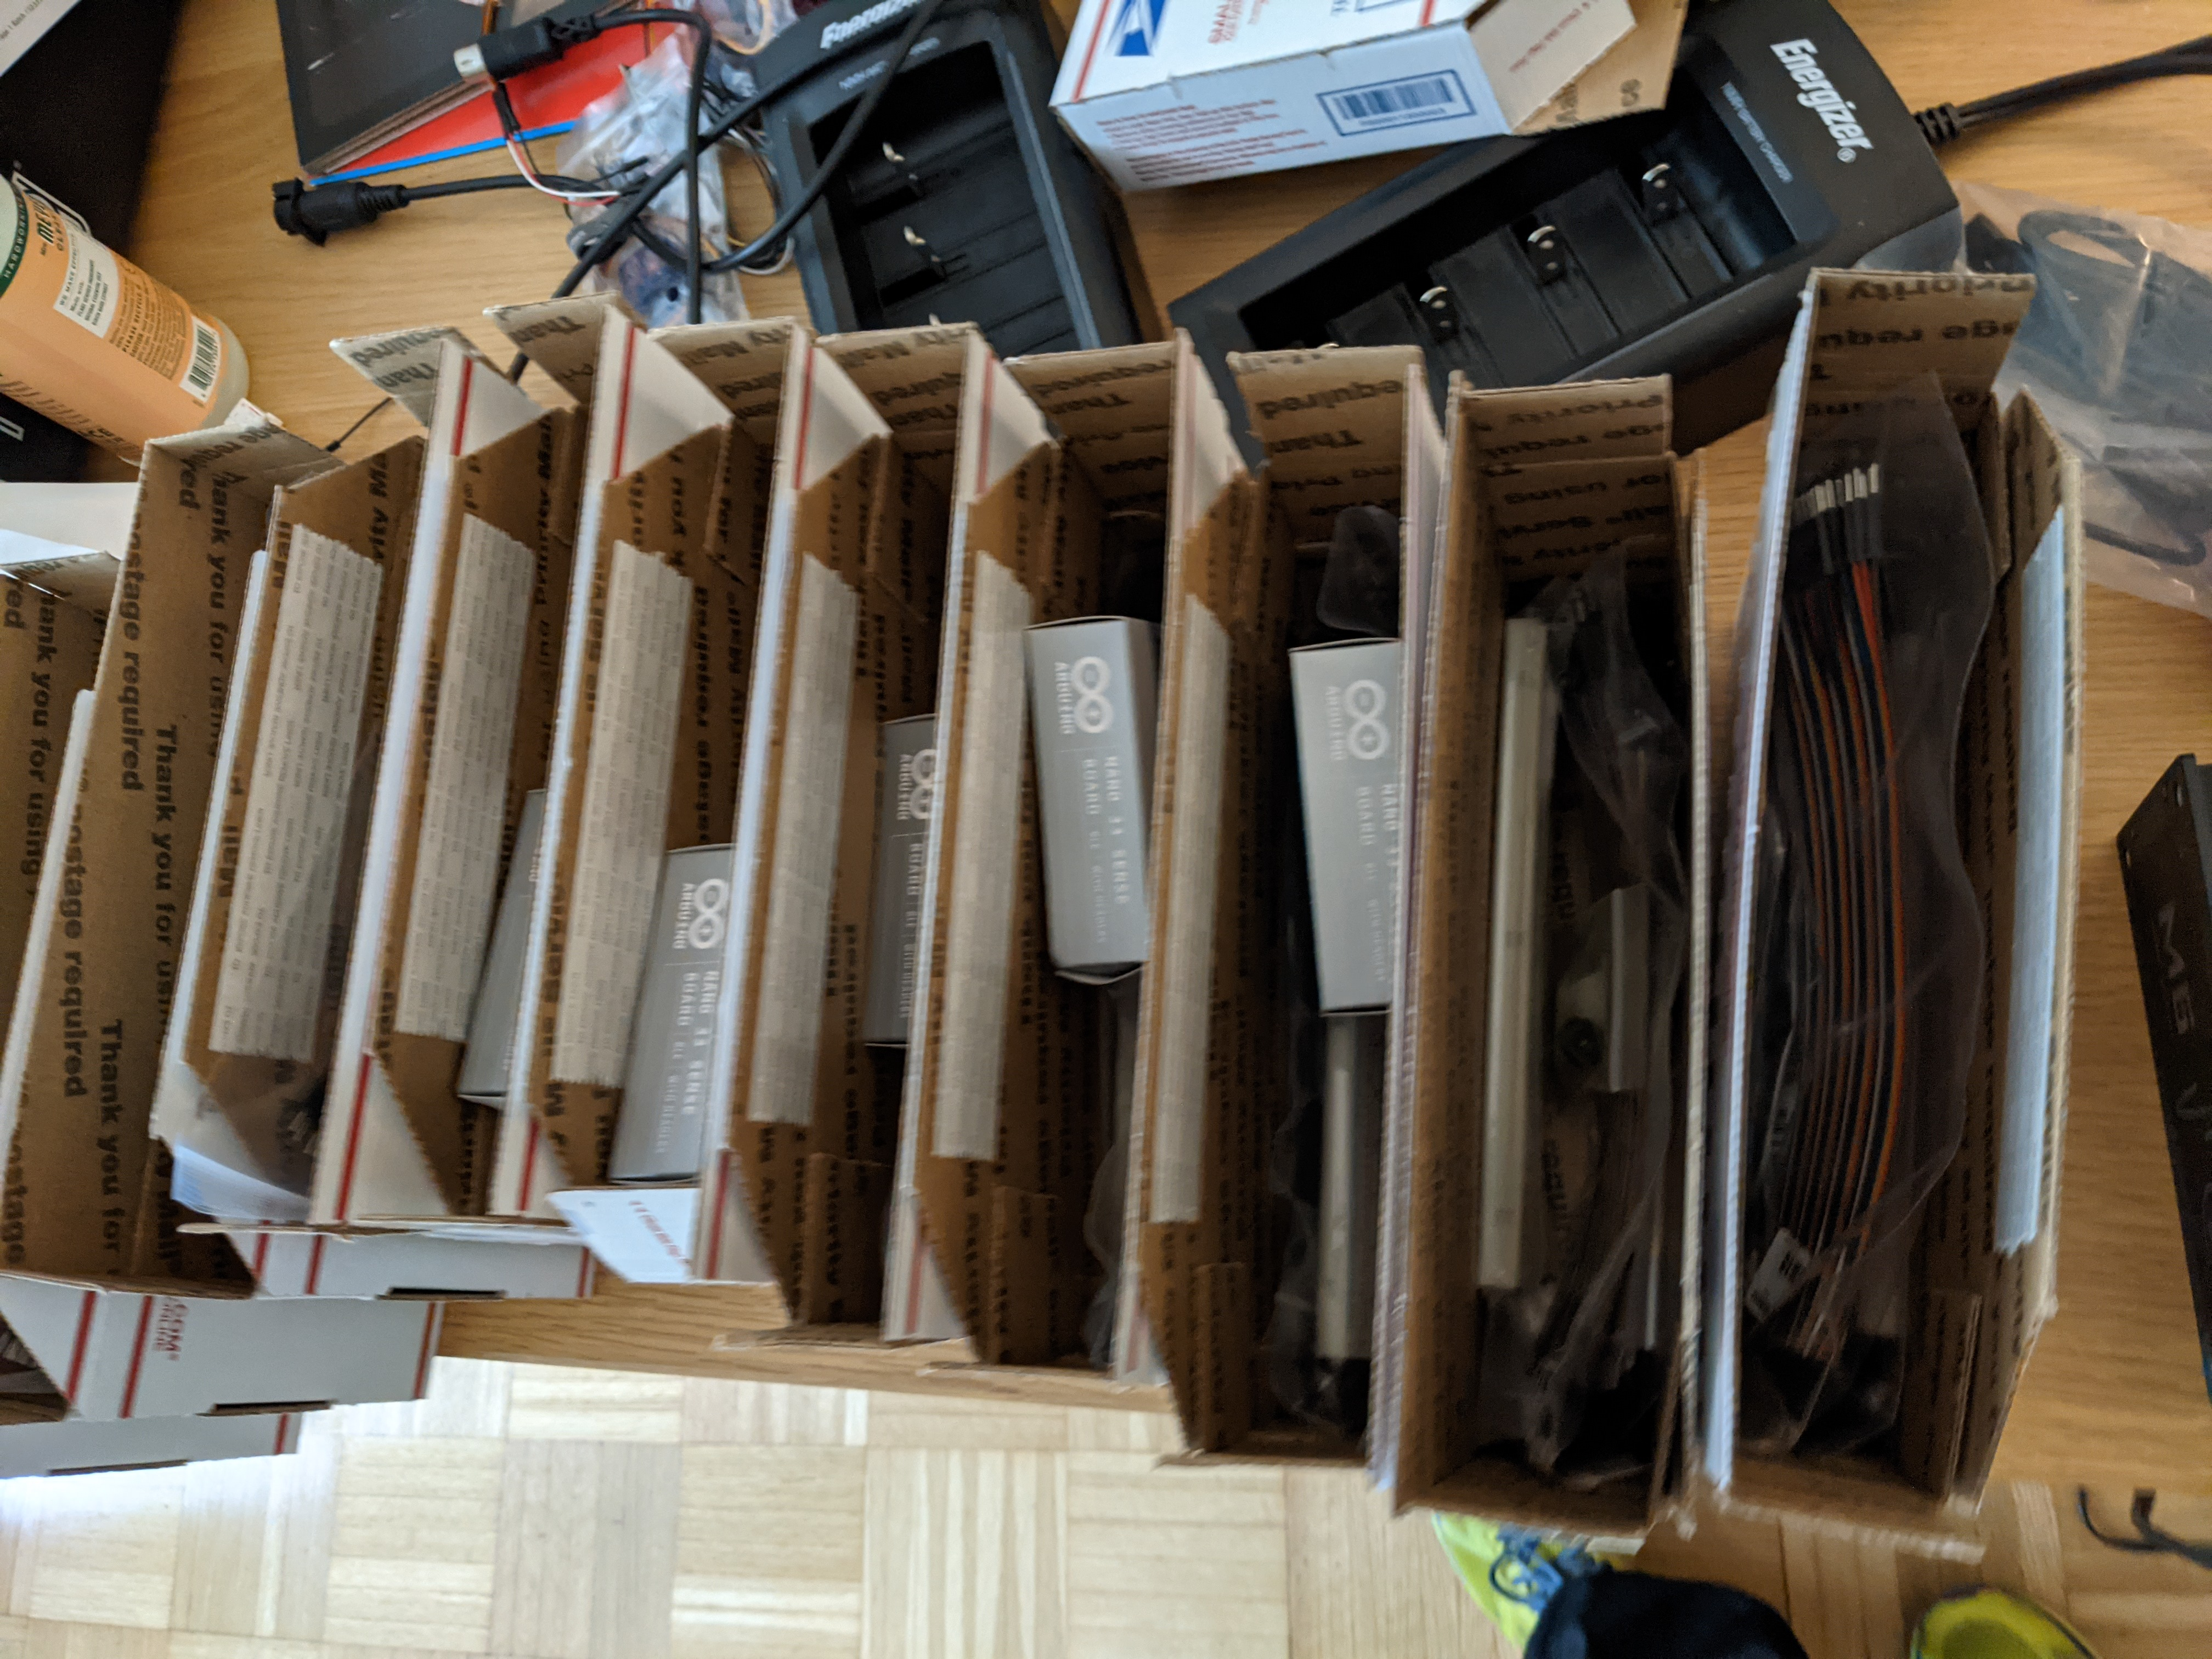
\includegraphics[width=0.75\linewidth,height=0.25\textheight,keepaspectratio]{images/workshop-packages.jpg}
	\caption{Workshop packages}
	\caption*{Picture taken at home}
	\label{fig:workshop-packages}
      \end{figure}

For user testing and sharing this thesis, some workshops were conducted during TODO, with support from a grant at CAMIT for teaching the workshops in English in USA, and in Chile in Spanish, remotely over teleconferencing software and after being approved by the MIT COUHES TODO explain.

The workshop instructions are documented on the docs/ folder of the repository available at https://github.com/montoyamoraga/tiny-trainable-instruments

Each workshop consists of 2 sessions of 2 hours each, spread over a weekend.

In the first session we will first help people with installation of the software, and then move on to start wiring the materials on the electronic breadboard material. We will concentrate on the simpler examples with color input. We will also collect data of gesture and speech to create custom databases and use them to train other slow machine learning models, that will keep on running on the student's workshops after the workshop is over.

On the second session we will use the result of the trained models to create more advanced instruments that react to gesture and speech. We will also show the participants the other 
 


\section{Multimedia documentation}

TODO: upload a collection of examples made by people who came to the workshops, featuring the software library and what they learned.
